\subsection{Modeling}
\label{sec:modeling}

\subsubsection{State Machines and Their Verification}
\danielle{Needs this? Check later. } A finite state machine (or finite state automaton) is a mathematical model of computation and consists of states, represented by nodes, and transitions between them, represented by directed edges. The change from one state to another is called a {\em transition}. The abstract machine can be in exactly one of a finite number of states at a time (hence, finite). \danielle{make figure?}

An infinite state machine has much more power in representation due to the ability to deal with infinite states. In domains like model checking, this is required since many of the variables used are from infinite domains (e.g., real numbers, integers). The expressive capabilities of set notation and predicate logic allow finite strings to represent these infinite states. For example, the infinite set of integers greater than zero is described succintly as: $\{x \in \mathbb{Z} : x > 0\}$. 

Abstracting a program or system with respect to a state machine is great, but without being able to reason about that abstraction, it is nothing more than slightly interesting. Information commonly required of a state machine representation is if a given state is {\em reachable}. In other words, reachability determines if is there a sequence of transitions that can lead to a given state. 

Model checkers often utilize the expressive power of state machines to verify specifications. One such example important to this thesis is JKind~\cite{2017arXiv171201222G}, an infinite state model checker. Verification of the program is based on {\em k-induction} (see Section~\ref{subsubsec:kInd}) and property directed reachability using a back-end SMT solver, e.g., Z3~\cite{z3}, SMTInterpol~\cite{smtInterpol}.

\subsubsection{Transition Systems}
Informally, a transition system is a model of states and transitions between them. Intuitively, finite automata are like transition systems with additional constraints, for instance, defined start and final states. Transition systems are directed graphs with nodes representing reachable states and edges representing transitions between them. They may also be defined with a mapping function that assigns labels to each node; in the context of model checking, these labels are often properties which must hold in the corresponding state.

Labeled transition systems are used extensively in model checking and will be mentioned within that context in later sections. There is much that could be said about transition systems, but for the purpose of this body of work, it is unnecessary. More information about transition systems and their relation to safety analysis and model checking can be found in the comprehensive book written by Bozzano and Villafiorita, Design and Safety Assessment of Critical Systems~\cite{Bozzano:2010:DSA:1951720}.

\textbf{$k$-induction}
\label{subsubsec:kInd}
The $k$-induction method was introduced as a technique for SAT-based verification of finite and infinite state transition systems~\cite{sheeran2000checking}. Let $I(s)$ and $T(s, s_0)$ be formulae encoding the initial states and transition relation for a system over sets of propositional state variables $s$ and $s_0$. Additionally, let $P(s)$ be a formula that represents the states satisfying a safety property and $k$ a positive integer. To prove the safety property $P$ by $k$-induction, there are two steps, the base case and the induction case. The base case must show that $P$ holds in all states reachable from an initial state within $k$ steps, or transitions. More formally, the base case must show that the following formula is unsatisfiable:

\begin{center}
$I(s_1) \land T(s_1, s_2) \land \cdots \land T(s_{k−1}, s_k) \land (\overline{P(s_1)} \lor \cdots \lor \overline{P(s_k)})$
\end{center}

The induction step must show that whenever $P$ holds in $k$ consecutive states, $s_1, \ldots, s_k$, $P$ also holds in the next state $s_{k+1}$ of the system. This is done by showing that the step case formula is unsatisfiable:

\begin{center}
$P(s_1) \land T(s_1, s_2) \land \cdots \land P(s_k) \land T(s_{k}, s_{k+1}) \land \overline{P(s_{k+1})}$
\end{center}

Ever since $k$-induction was introduced for the purpose of verification of state machines, various methods came about of either combining these two proof steps into one~\cite{donaldson2011software} or performing them in parallel~\cite{kahsai2011pkind}. \\

\danielle{Putting this here for now. Probably cut later.}

\subsubsection{Ordered Binary Decision Diagrams}
A Binary Decision Diagram (BDD) is a data structure used to encode Boolean formulae.
\begin{figure}[htbp]
        \center{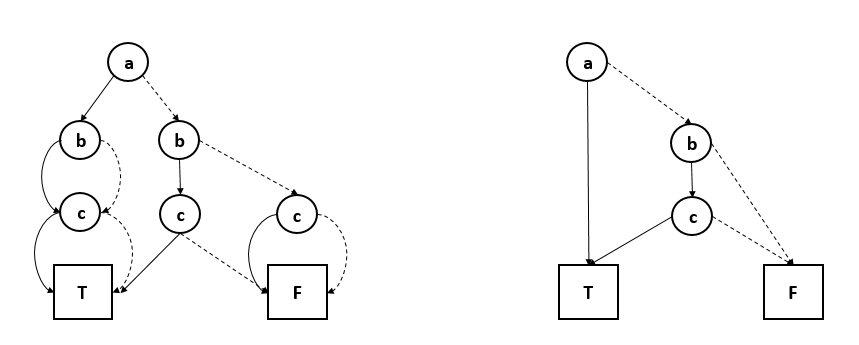
\includegraphics[width=0.8\textwidth] {images/bdd.png}}
        \caption{\label{fig:bdd} Binary Decision Diagrams of the Formula $a \lor (b \land c)$}
\end{figure}
As shown in Figure~\ref{fig:bdd}, it is a rooted, directed, acyclic graph with internal decision nodes and two terminal nodes (\textit{true} and \textit{false}). Each of the decision nodes is labeled with a Boolean variable and has two child nodes, low child and high child. The edge from a node to its low child represents the assignment of \textit{false}, likewise the edge to the high child represents the assignment of \textit{true}. The BDD is called \textit{ordered} if different variables appear in the same order on all paths from the root. Intuitively, following a path from the root to the \textit{true} terminal node represents a valid assignment to the Boolean formula (invalid in the case of ending on the \textit{false} terminal node). 

BDDs are reduced by the removal of isomorphic subgraphs. The BDD shown on the right of Figure~\ref{fig:bdd} is the reduced form of the BDD on the left.